\documentclass{beamer}

\mode<presentation> {
  \usetheme{Singapore}
  %\setbeamercovered{transparent}
  %\usecolortheme{wolverine}
}

\usepackage{palatino}
\usepackage{graphicx}

\AtBeginSection[]
{
  \begin{frame}
    \frametitle{Table of Contents}
    \tableofcontents[currentsection]
  \end{frame}
}

\title{Identifying License Plates Ids with Hidden Markov
    Models}
\author{ James Pritts and Ondrej Hrstka }
\institute[CTU FEE]{Czech technical university - Faculty of Electrical Engineering}
\date{13.2.2012}

\begin{document}
\begin{frame}
  \titlepage
\end{frame}


\section{Introduction}

\begin{frame}
  \frametitle{Problem statement}
JAMES  
  
  The problem is to report the unique identifying string of characters,
called the \emph{vehicle-id}, of a license plate.  Provided are images
of license plates that have been segmented and ortho-rectified. A
subset of these images each have the following corresponding
annotations: a top and bottom boundary that delimits the
\emph{vehicle-id} within the segmented license plate, a bounding box
of each character and white-space interval that comprises the
\emph{vehicle-id}, and a character label for each bounding box that
contains a character.  We assume that the font of all characters
across license plates is identical, and we refer to a particular
character of the font set as a glyph.

\end{frame}

\begin{frame}
  \frametitle{Model definition}
  JAMES
\[S =
\left(\,\dots,\text{w},\text{A}_1,\text{A}_2,\ldots,\text{A}_{m},\text{w},\text{w},\text{w},\text{T}_1,\text{T}_2,\ldots\,\right).\]
\end{frame}

\section{Learning the model}

\begin{frame}
  \frametitle{Input dataset}
  Input dataset is contains 5000 annotated examples. Each example is structure containing:
\begin{itemize}
  \item Original license plate images
  \item Cropped and normalized image
  \item Characters string with bounding boxes for each character.
\end{itemize}

\begin{figure}
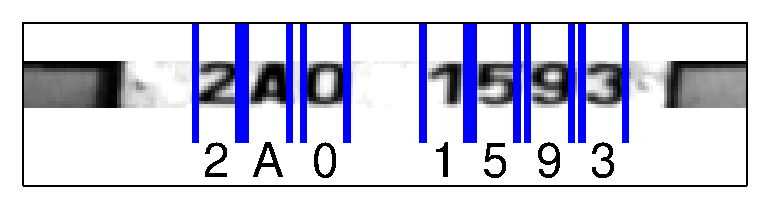
\includegraphics[width=\linewidth]{pics/input_example.eps}
\caption{Example of annotated input data. Normalized image displayed.}
\label{fig:distribution}
\end{figure}

\end{frame}

\begin{frame}
  \frametitle{Learning the emission probabilities}
	Emission probabilities of the model were learened using EM algorithm.
  
\end{frame}

\begin{frame}
  \frametitle{Learning the emission probabilities}
\begin{block}{E-step}
	\[
  p(x_{ij} \mid c=f, s_j)_d^{t+1} = \frac{\mathcal{N}(\sigma_1^t,\mu_1^t)\gamma_{is_j}^t}{\mathcal{N}(\sigma_1^t,\mu_1^t)\gamma_{is_j}^t+\mathcal{N}(\sigma_2^t,\mu_2^t)(1-\gamma_{is_j}^t)}
\]
	\end{block}

\begin{block}{M-step}
\[
  \gamma_{is_j}^{t+1} = \frac{\sum_{d \in \mathcal{D}} p(x_{ij} \mid c=f, s_j)_d^{t+1}}{\sum_{d \in \mathcal{D}} p(x_{ij} \mid c=f, s_j)_d^{t+1} + \sum_{d \in \mathcal{D}} (1-p(x_{ij} \mid c=b, s_j)_d^{t+1})}
\]
\[
  \sigma_1^{t+1} = \frac{\sum_{i,j} \sum_{d \in \mathcal{D}} x_{d, i,j} p(x_{ij} \mid c=f, s_j)_d^{t+1} }{\sum_{i,j} \sum_{d \in \mathcal{D}} p(x_{ij} \mid c=f, s_j)_d^{t+1}}
\]  
\end{block}  
\end{frame}

\begin{frame}
  \frametitle{Learning the emission probabilities}
\begin{itemize}
\item Stopping criterion is relative
\item  $|1-\frac{\sigma_1^{t+1}}{\sigma_1^{t}}| < \epsilon \wedge |1-\frac{\sigma_2^{t+1}}{\sigma_2^{t}}| < \epsilon$
\item$\epsilon$ has been set to value $10^{-5}$
\end{itemize}  
\end{frame}

\begin{frame}
  \frametitle{Learned templates}
\begin{figure}[htp]
\centering
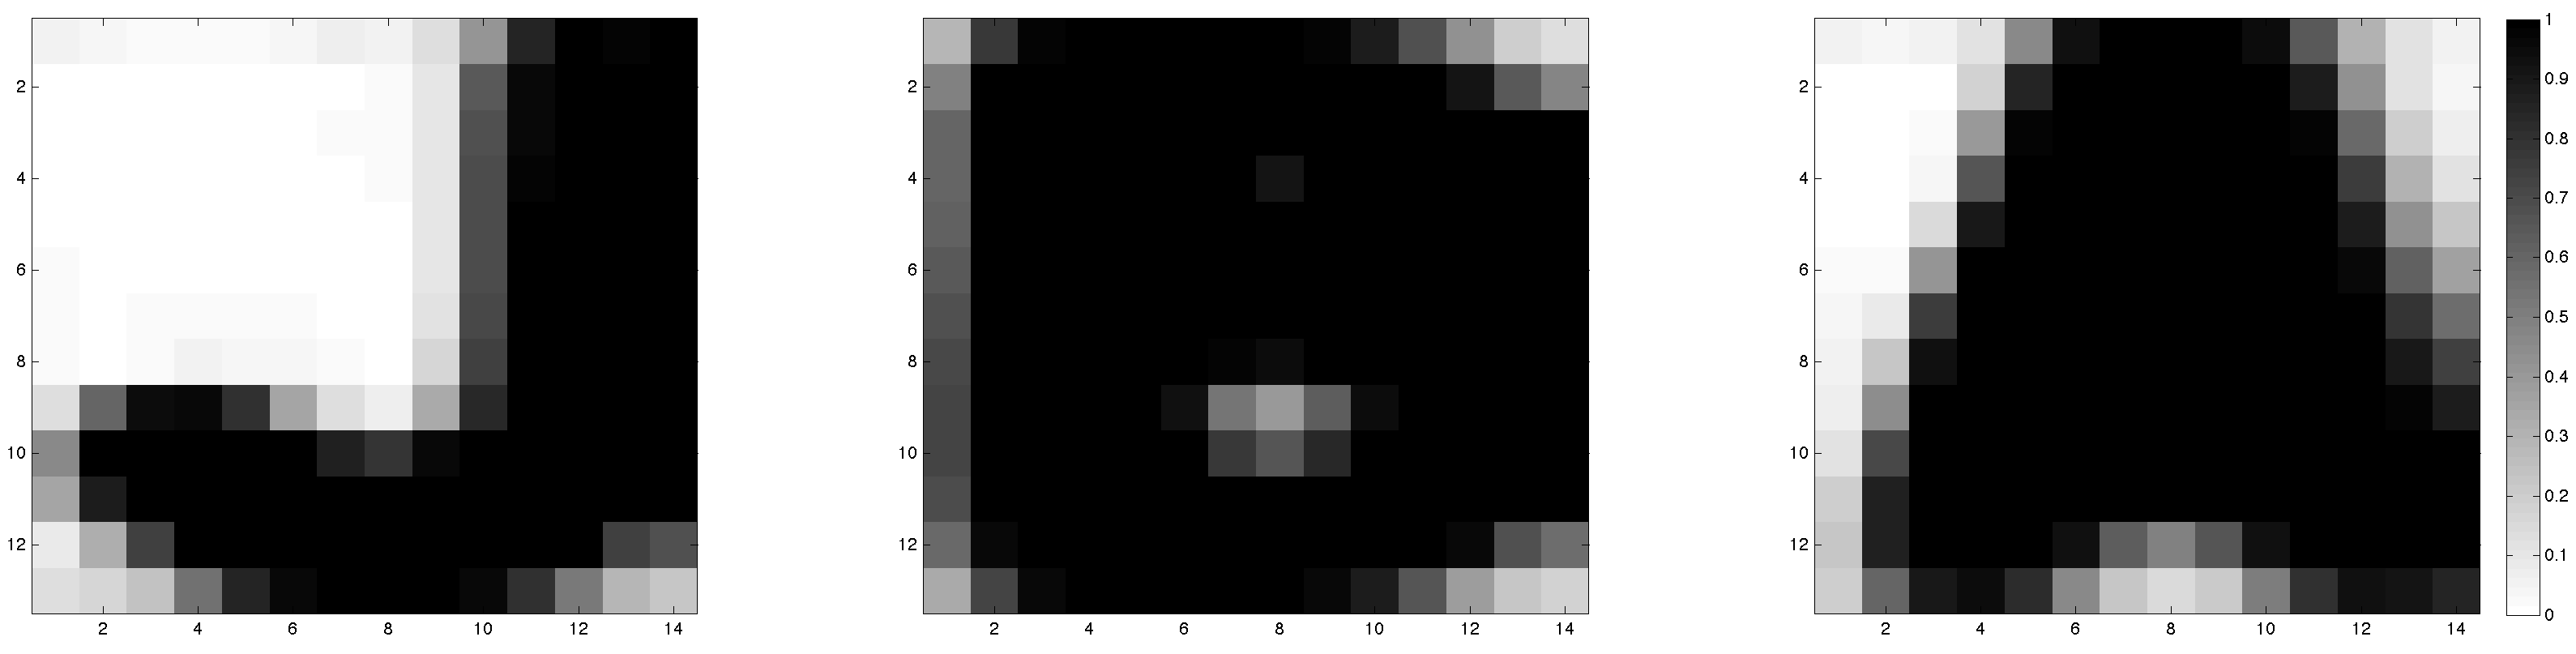
\includegraphics[width=\linewidth]{pics/jba.png}
\caption{Learned templates of \texttt{J}, \texttt{B} and
  \texttt{A}. Intensity corresponds to the prior probability for being
  a foreground pixel.}
\label{fig:templates}
\end{figure}
\end{frame}




\begin{frame}
  \frametitle{Setting the transition probabilities}
  JAMES
\end{frame}


\begin{frame}
  \frametitle{Inference}
  JAMES
\end{frame}

\section{Evaluation}
\begin{frame}
  \frametitle{Evaluation}
  
\end{frame}

\begin{frame}
  \frametitle{Conclusions}
\end{frame}

\end{document}
